\documentclass[a4paper,11pt]{article}
\usepackage{graphicx}
\usepackage[margin=.5in]{geometry}
\begin{document}

\listoffigures


\begin{figure}[h]
\centerline{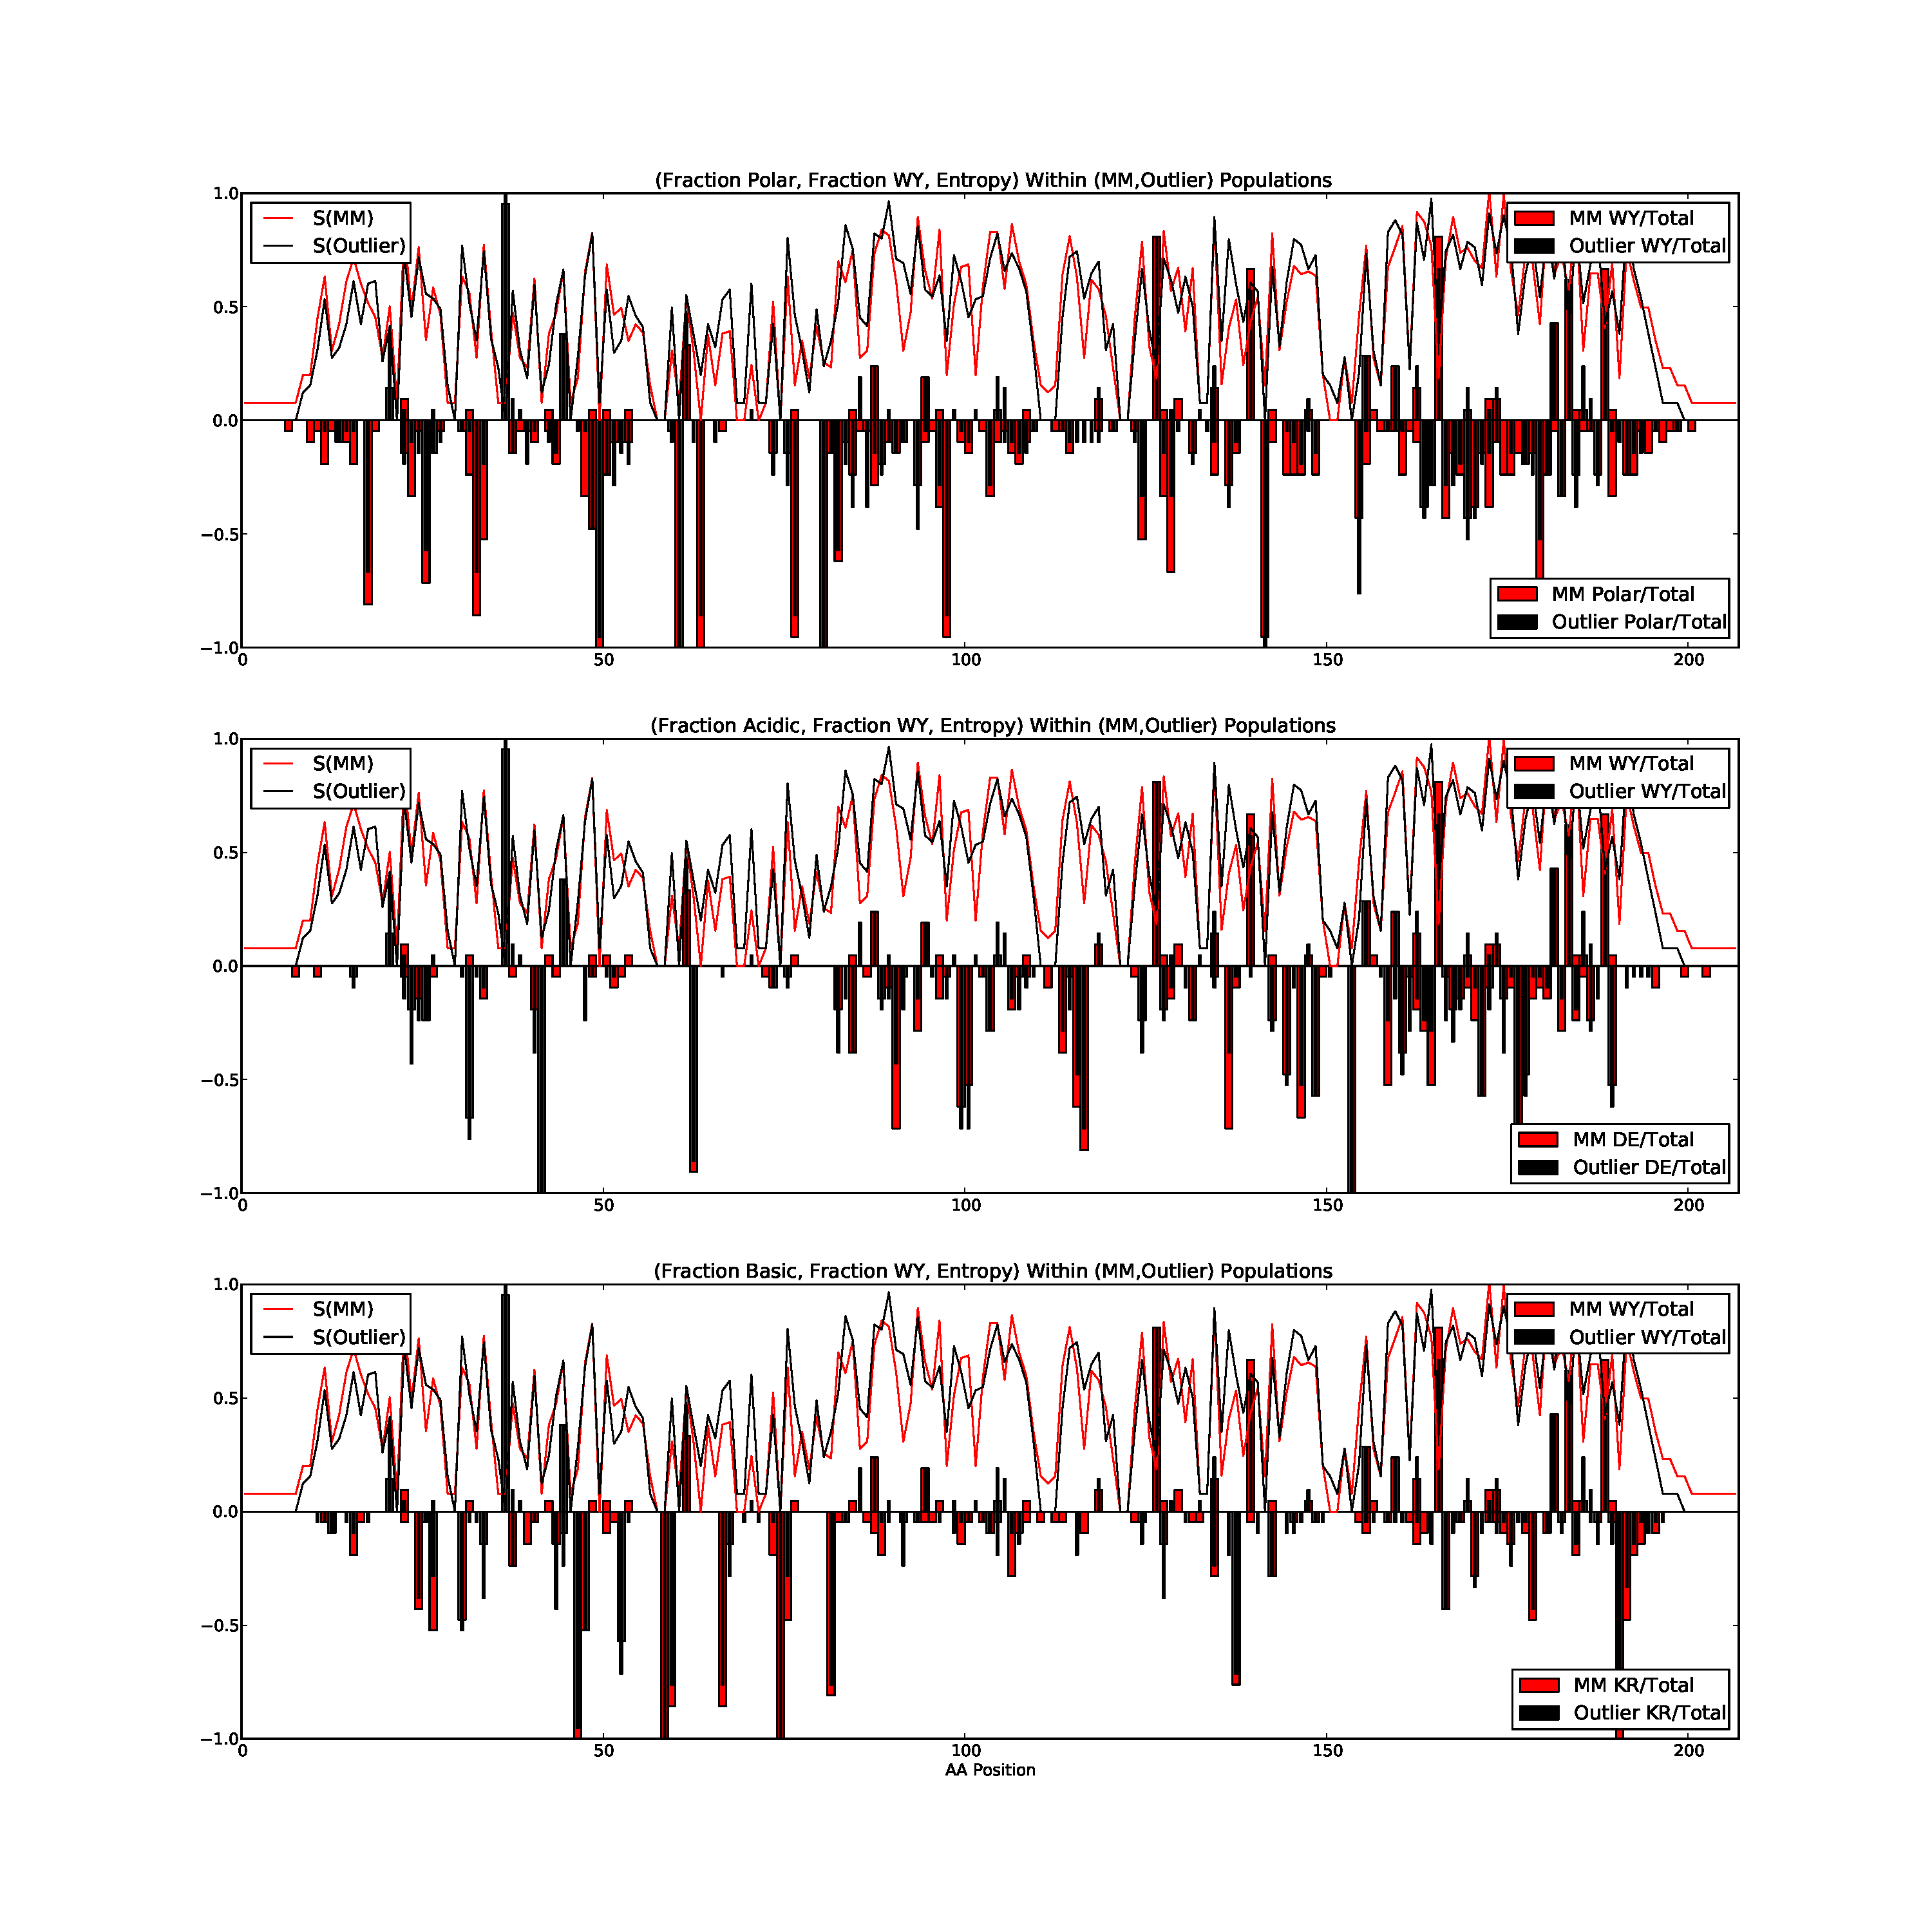
\includegraphics[width=8in]{AA+S.pdf}}
\caption[$S_{\rm red}$, $S_{\rm black}$, WY/Polar/Acidic/Basic Content vs Residue \#]{Entropy and fractional WY/Polar/Acidic/Basic content plotted as a function of position within the DHFR global alignment. Each variable (S, fractional WY content, etc) was plotted simultaneously for both the red grop (DHFR sequences which, upon introduction into E. Coli, conferred Michaelis-Menton obeying behavior) and the black group (DHFR sequences which did not). The entropy of each residue across different DHFR sequences was plotted as a line in the ordinal range [0,1.0] with 1.0 corresponding to 4 bits of entropy per residue per sequence. In the same ordinal range of [0,1.0], bars were drawn indicating the fraction of DHFR sequences in the respective red/black groups which contained W or Y residues at that location. Below the horizontal axis, a similar fractional content chart was created indicating the portion of red/black DHFR sequences containing polar, acidic, or basic residues at that location.}
\end{figure}



\begin{figure}[h]
\centerline{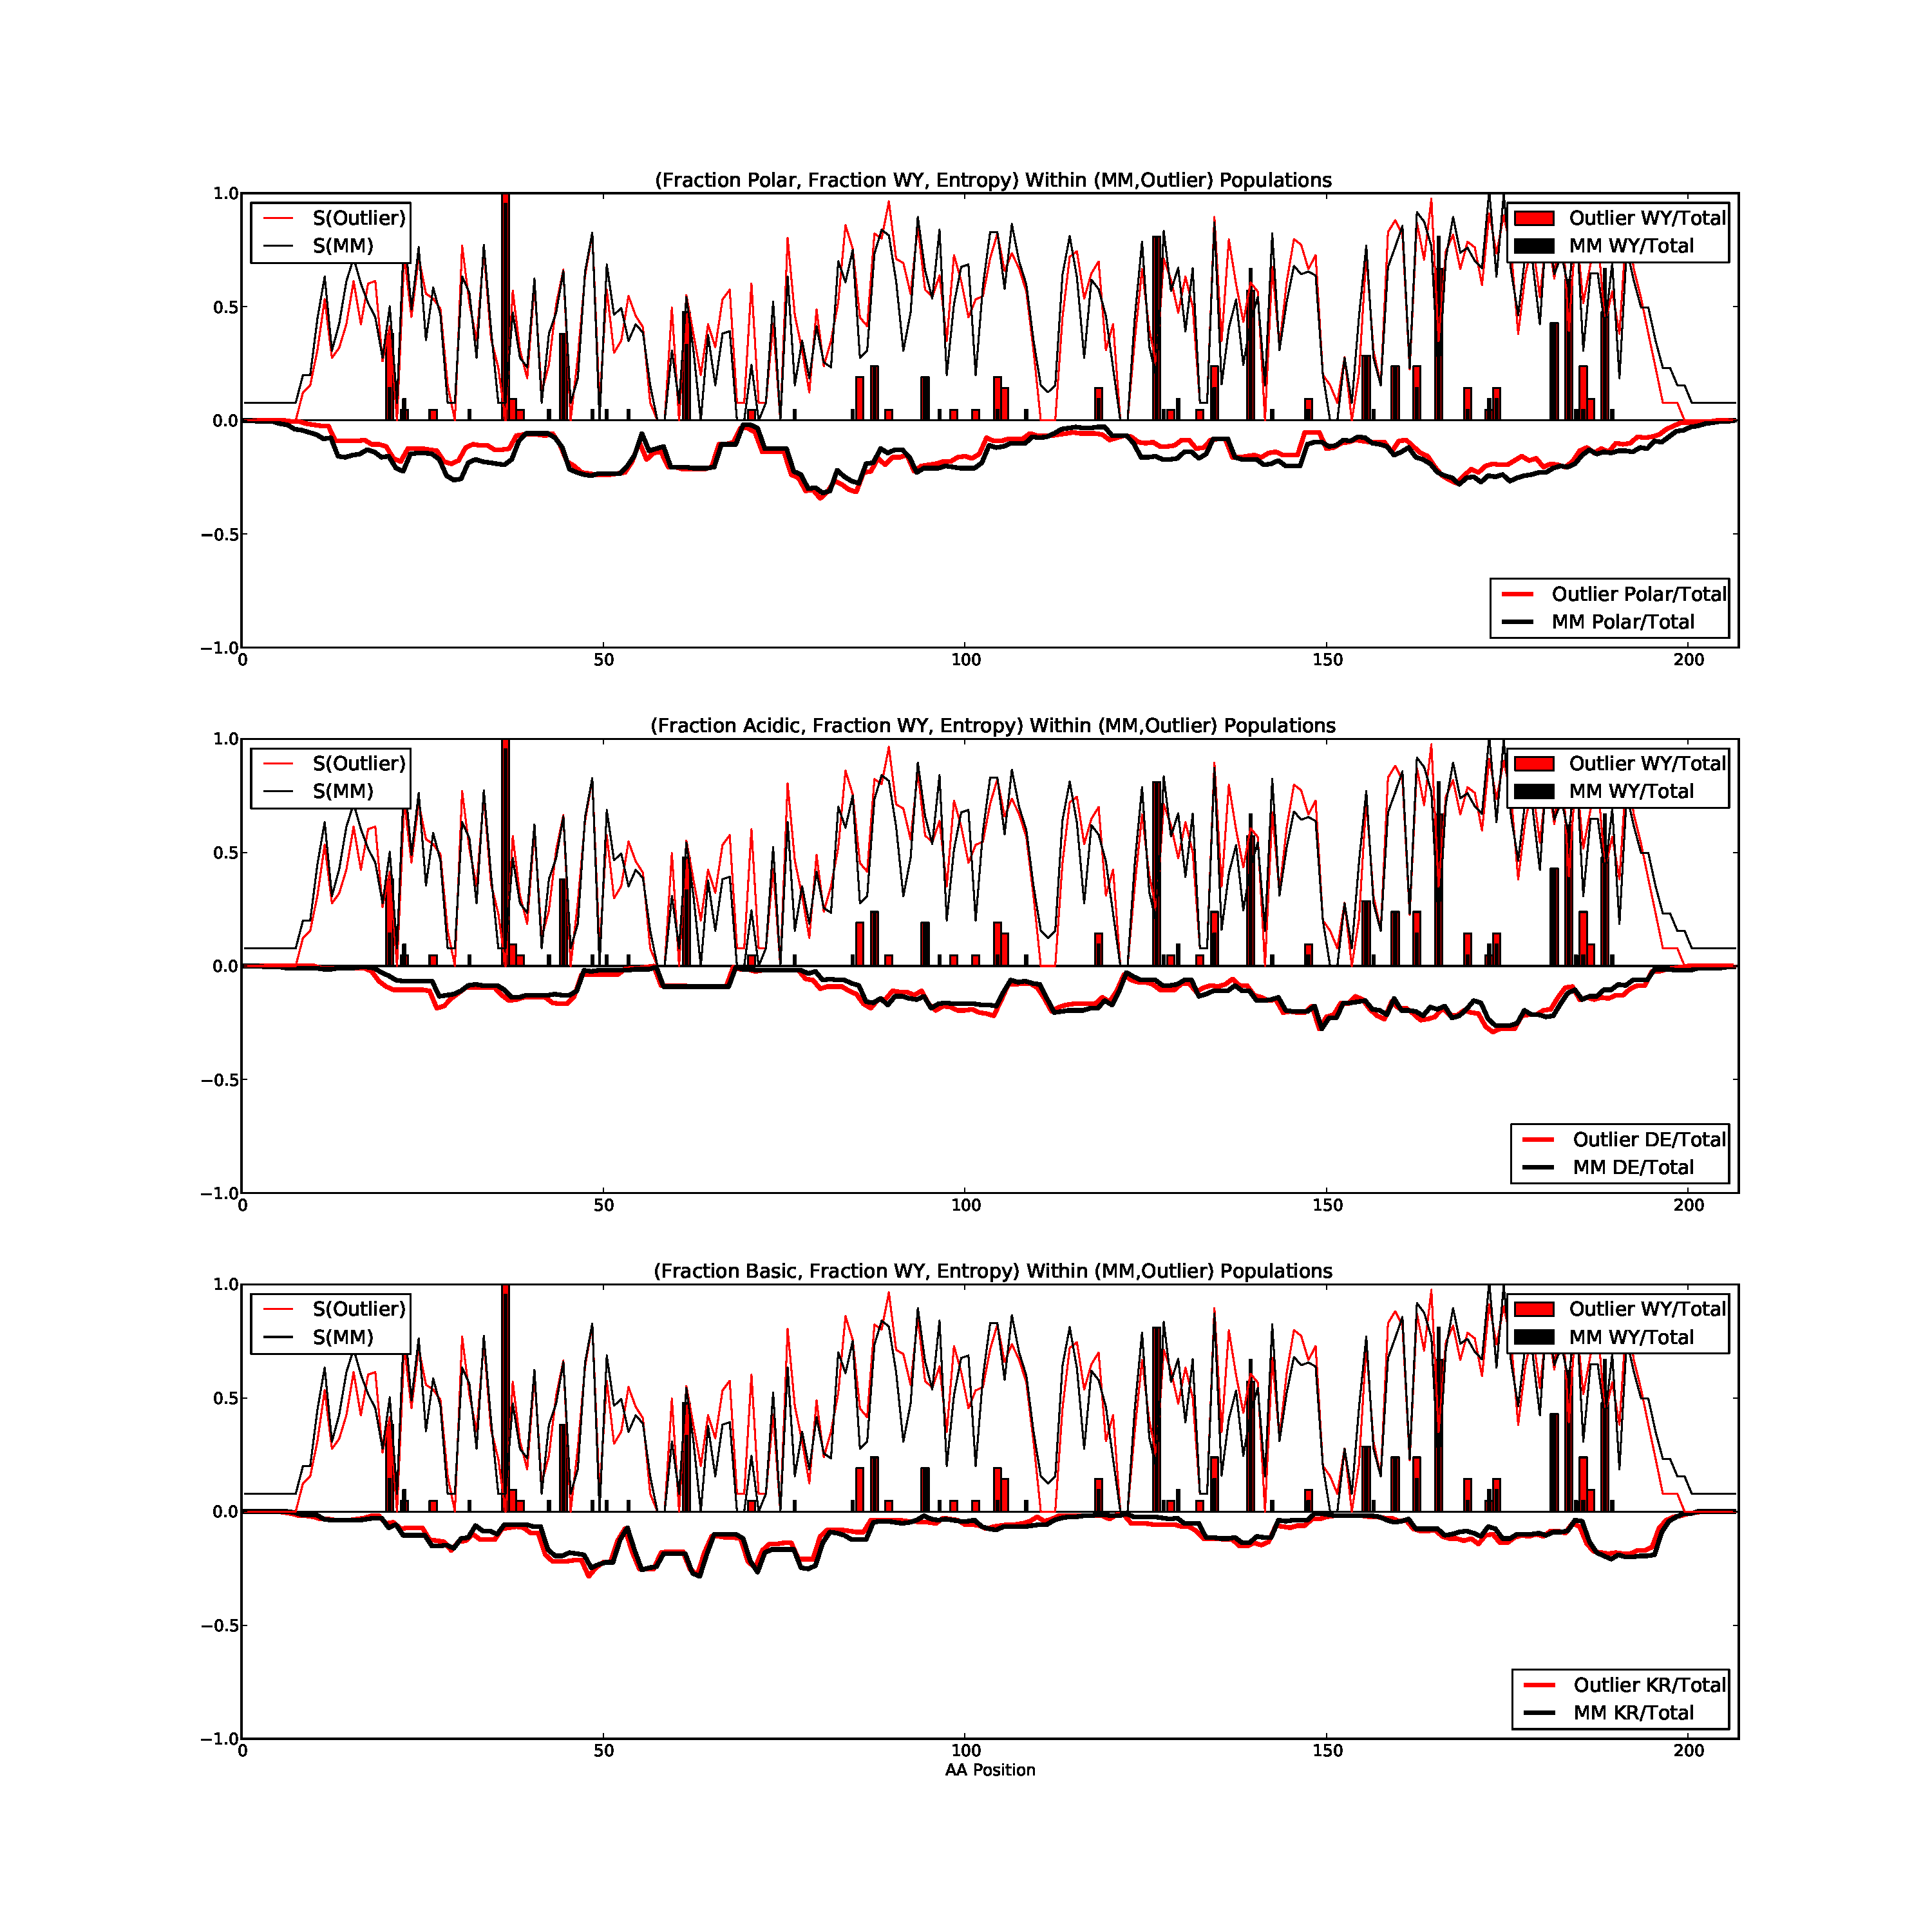
\includegraphics[width=8in]{AA+S_smooth.pdf}}
\caption[$S_{\rm red}$, $S_{\rm black}$, Moving-Average $S_{\rm red}$, Moving-Average $S_{\rm black}$, WY Content vs Residue \#]{Entropy and fractional WY/Polar/Acidic/Basic content plotted as a function of position within the DHFR global alignment. Each variable (S, fractional WY content, etc) was plotted simultaneously for both the red grop (DHFR sequences which, upon introduction into E. Coli, conferred Michaelis-Menton obeying behavior) and the black group (DHFR sequences which did not). The average entropy of each residue across DHFR sequences inside a 20 residue moving window was plotted as a line in the negative ordinal range [-1,0] with -1.0 corresponding to 4 bits of entropy per residue per sequence. Red/black residue entropy was plotted without a moving average in the positive ordinal range [0,1]. In the same ordinal range of [0,1.0], bars were drawn indicating the fraction of DHFR sequences in the respective red/black groups which contained W or Y residues at that location.}
\end{figure}




\begin{figure}[a]
\centerline{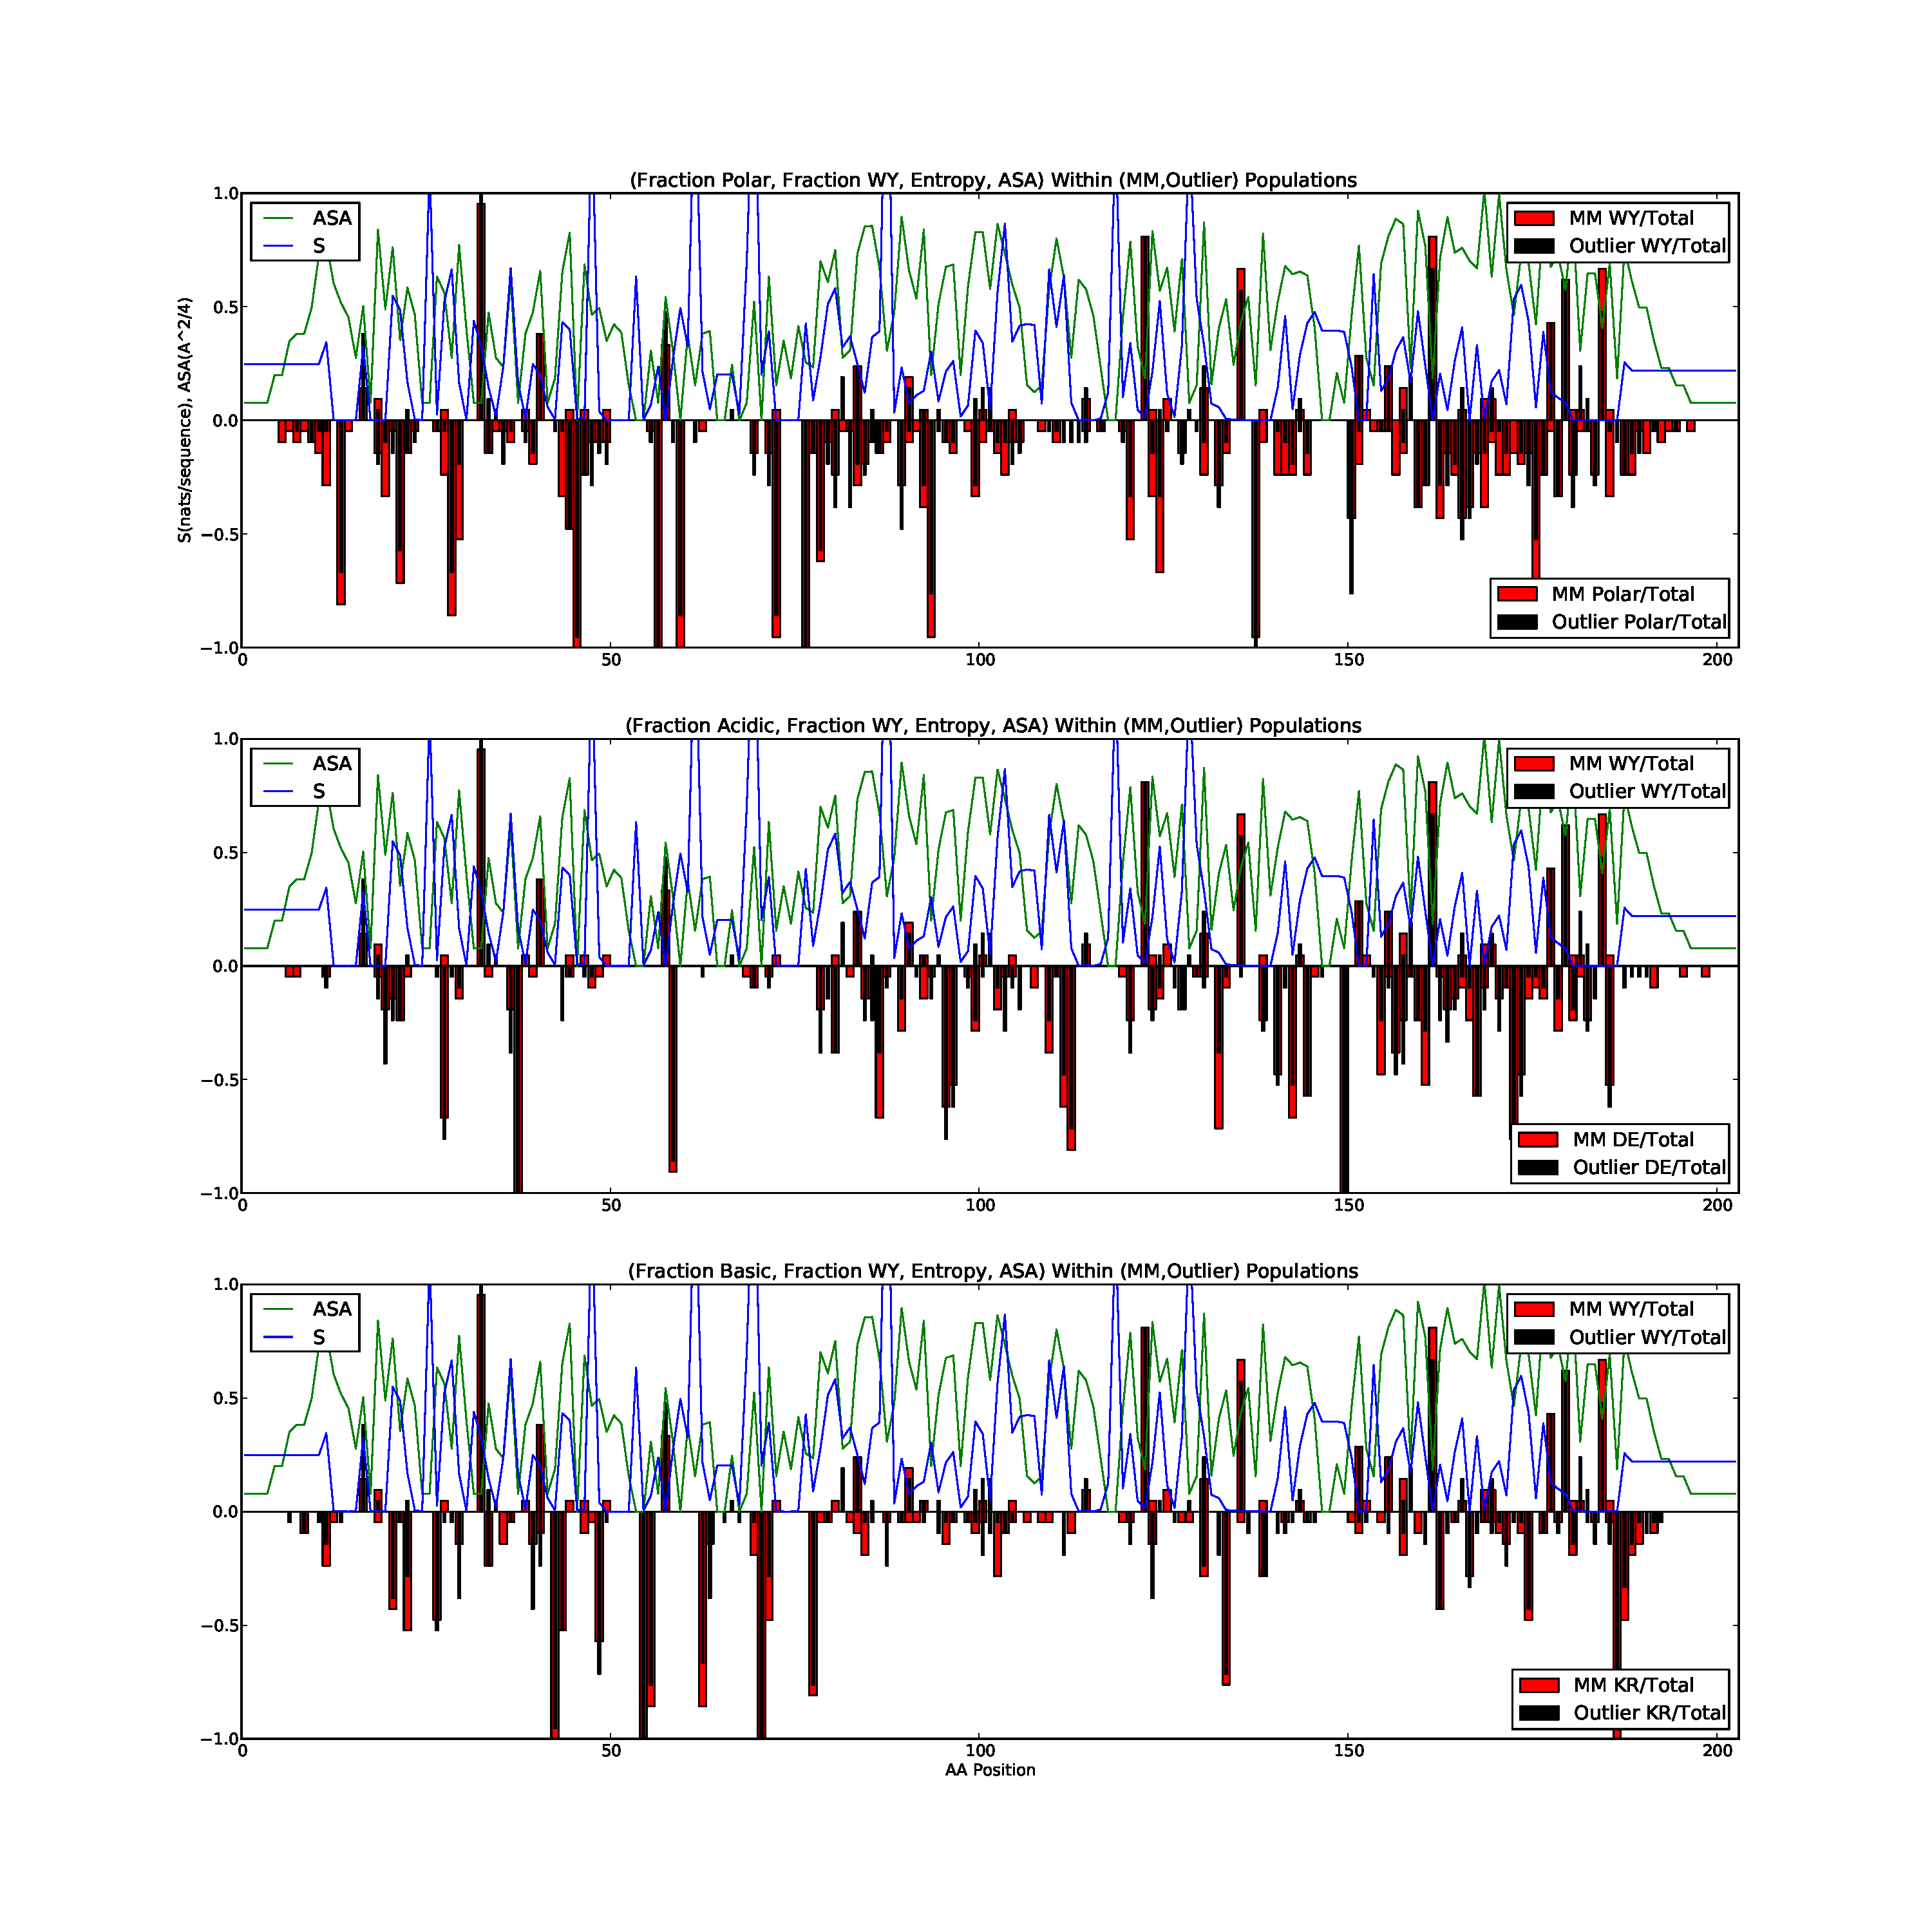
\includegraphics[width=8in]{AA+S+ASA.pdf}}
\caption[$S_{\rm all}$, $ASA_{\rm all}$, WY/Polar/Acidic/Basic Content vs Residue \#]{Normalized Accessible Surface Area and Entropy were averaged over DHFR structures and plotted as a function of residue \#. For clarity, these averages were taken over all DHFR, rather than separately over those belonging to the red (Michaelis-Menton obeying) and black (outlier) groups since the noise level drowns out the difference between the two groups without smoothing over the residue-\# axis. A 1.0 ordinal value corresponds to an entropy of 4 bits (per residue per sequence) or an ASA of 50\% of the highest observed ASA (HOA) within a large training set. The fractional content of W,Y residues at each position within the red and black groups was plotted using red and black bars in the ordinal range $[0,1.0]$ while the fractional content of an additional class of residue (polar, acidic, or basic) was plotted in the same format but in the ordinal range $[-1.0,0]$ using downward-facing bars.}
\end{figure}



\begin{figure}[a]
\centerline{\includegraphics[width=8in]{AA+S+ASA_smooth.pdf}}
\caption[Moving-Averages of $S_{\rm all}$, $ASA_{\rm all}$, WY/Polar/Acidic/Basic Content vs Residue \#]{Normalized Accessible Surface Area and Entropy were averaged over red/black DHFR sequences, \textbf{then over residue\# using a 10 residue sliding window} and plotted as lines. A 1.0 ordinal value corresponds to an entropy of 4 bits (per residue per sequence) or an ASA of 50\% of the highest observed ASA (HOA) within a large training set. The fractional content of W,Y residues at each position within the red and black groups was plotted using red and black bars in the ordinal range $[0,1.0]$ while the fractional content of an additional class of residue (polar, acidic, or basic) was plotted in the same format in the ordinal range $[-1.0,0]$ using downward-facing bars.}
\end{figure}


\begin{figure}
\centerline{\includegraphics[width=8in]{window_an.pdf}}
\caption[Moving Averages of $S_{\rm red},S_{\rm black},ASA_{\rm red},ASA_{\rm 
black}$ for Windows of (5,10,20) Residues]{Entropy per residue per sequence was measured in bits/4 and plotted in the $[0,1]$ ordinal range for Michaelis-Menton obeying (red) and outlier (black) sequences. Accessible Surface Area was plotted in the $[-1,0]$ ordinal range, measured in units of HOA/2 (the Highest Observed ASA of the corresponding 3-residue environment in PDB), averaged over DHFR sequences. Both quantities were then subject to a moving average over the residue\# axis using a box window of length (5,10,20). Locations at which polar, acidic, basic, or WY residues composed $>25\%$ of the DHFR alignment ensemble were indicated by dots on the horizontal axis. One notable feature that varies under window choice is hte effect of spikes in the raw normalized ASA trace (see Figure 3) corresponding to glycine residues (presumably in loops).}
\end{figure}



\begin{figure}
\centerline{\includegraphics[width=8in]{asa_hist.pdf}}
\caption[Histogram of (Polar,Acidic,Basic) ASA over MM, Outlier Groups]{The Accessible Surface Area of polar, acidic, and basic residues within the DHFR structures which obeyed MM kinetics (red) and those that did not (black) were computed and a continuous histogram (kernel density estimate) for each class was plotted over normalized ASA. A continuous histogram was used in order to ensure that the result was translation invariant. The normalization is such that each histogram integrates to 1.}
\end{figure}


\begin{figure}
\centerline{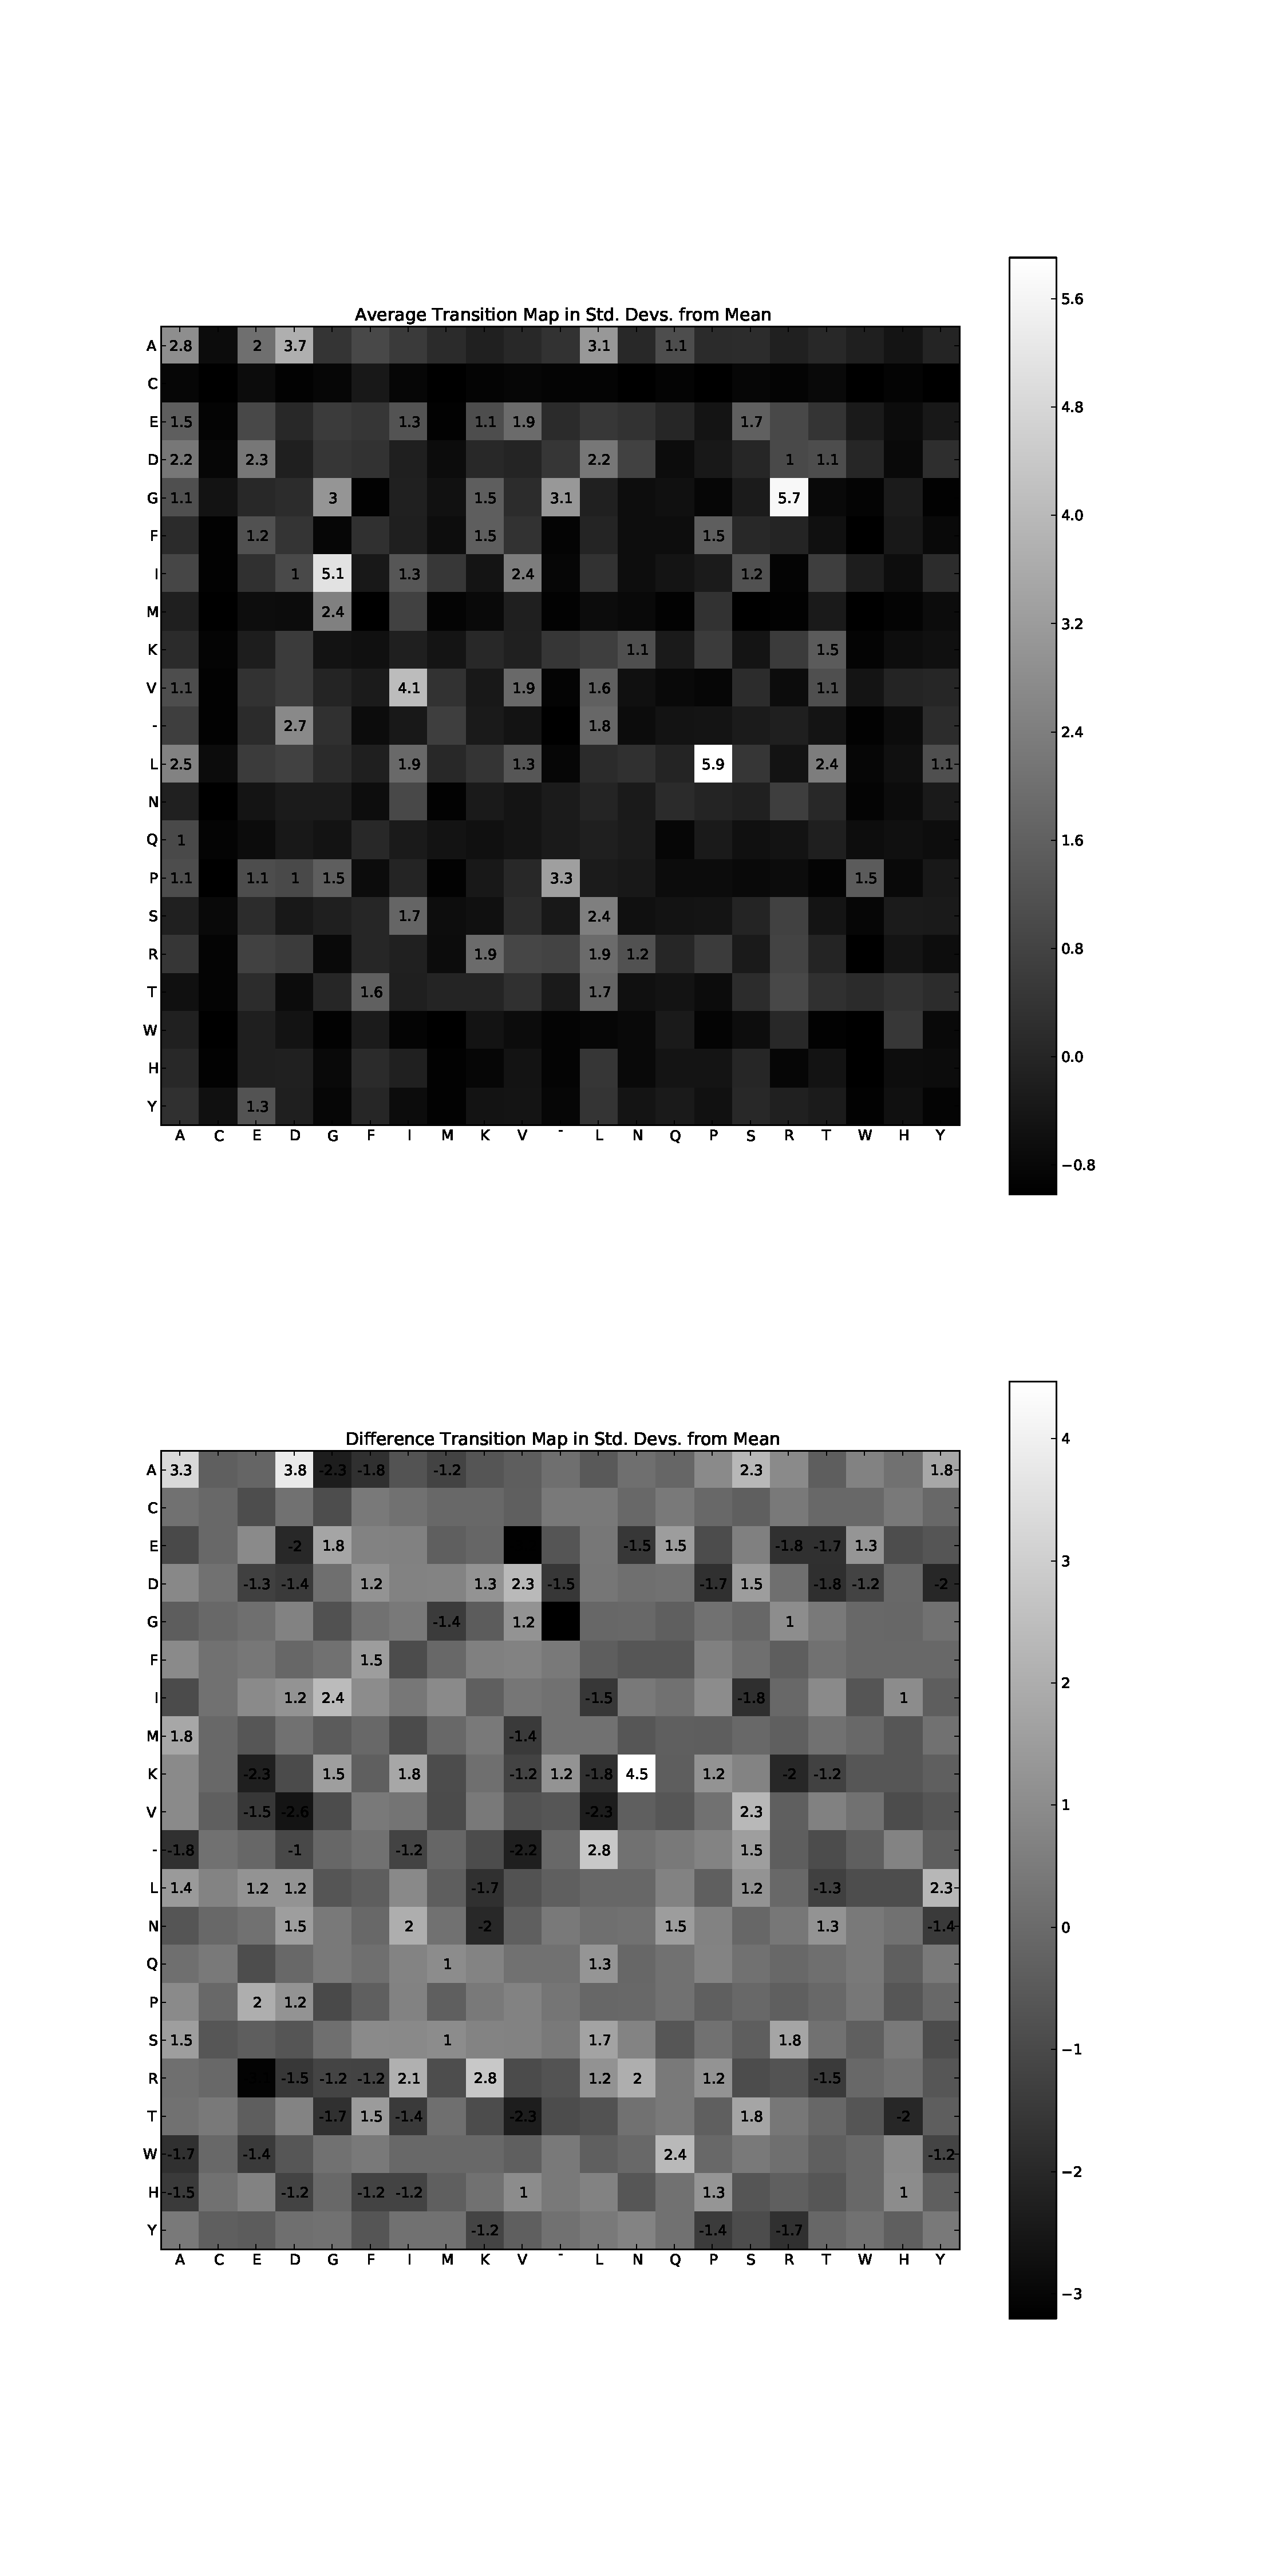
\includegraphics[width=8in]{transitions.pdf}}
\caption[Amino Acid Transition Matrix]{The transition counts between amino acids in sequences of the DHFR structures which obeyed MM kinetics (red) and those that did not (black) were computed and displayed in a table. Rows correspond to the amino acid closer to the n-terminal end of the protein. For the purposes of computation, gaps were treated as additional amino acids. Since there were a different number of sequences in the red and black groups, the numbers in the black group were renormalized and rounded off to integers. The difference between the number of observed AA transitions of a given type between red/black DHFR sequences was then computed and plotted in purple. A continuous histogram of these values was provided to assess the significance of outliers.}
\end{figure}

\begin{figure}
\centerline{\includegraphics[width=8in]{transitions_normed.pdf}}
\caption[Amino Acid Transition Matrix with Normalized Differences]{The transition counts between amino acids in sequences of the DHFR structures which obeyed MM kinetics (red) and those that did not (black) were computed and displayed in a table. Rows correspond to the amino acid closer to the n-terminal end of the protein. For the purposes of computation, gaps were treated as additional amino acids. Since there were a different number of sequences in the red and black groups, the numbers in the black group were renormalized and rounded off to integers. The difference between the number of observed AA transitions of a given type between red/black DHFR sequences was then computed and plotted in purple, after being divided by the average transition count to control for the difference in absolute transition propensities. A continuous histogram of these values was provided to assess the significance of outliers.}
\end{figure}



\end{document}